\documentclass[conference, 9pt]{IEEEtran}
\usepackage{amsmath}
\usepackage{amssymb}
\usepackage{color}
\usepackage[font=footnotesize]{subfig}
% \usepackage{eqnarray}
\usepackage{algpseudocode}
\usepackage{varwidth}
\usepackage{paralist}
\usepackage{graphicx}
\usepackage{multirow}
\usepackage{listings}
\graphicspath{{figures/}}

% \renewcommand{\algorithmiccomment}[1]{\hfill\eqparbox{COMMENT}{\# #1}}

\usepackage{url}

% correct bad hyphenation here
\hyphenation{op-tical net-works semi-conduc-tor}


\usepackage{varwidth}
\usepackage{paralist}

% \setlength{\parskip}{1pt}
\setlength{\tabskip}{0em}
% \setlength{\parindent}{1em}
\newcommand{\startcompact}[1]{\par\vspace{-0.75em}\begin{#1}%
\allowdisplaybreaks\ignorespaces}
\newcommand{\stopcompact}[1]{\end{#1}\ignorespaces}

\definecolor{gray20}{gray}{0.20}

\newcommand{\gray}[1]{\color{gray20}{#1}}
\newcommand{\red}[1]{\textcolor{red}{#1}}
\newcommand{\green}[1]{\textcolor{green}{#1}}
\newcommand{\dgreen}[1]{\textcolor{green}{#1}}
\newcommand{\blue}[1]{\textcolor{blue}{#1}}

\begin{document} 

%\title{NoC-based Multi-FPGA Application Mapping:\\ A case study with Boolean Matrix-Vector Multiplication}
\title{NoC-based Multi-FPGA Application Mapping: A Case Study Accelerating Krylov Sequence Computations over GF(2)}
%\title{NoC-based Multi-FPGA Application Mapping: a case study with Krylov sequence computations over GF(2)}
% \title{Boolean Matrix Vector Multiplication:\\ A Case-study in NoC-based Multi-FPGA Application Mapping}
\maketitle 

\begin{abstract}

\end{abstract}

% \IEEEpeerreviewmaketitle

\section{Introduction}


\blue{
\subsection{Relevant focus areas for FSP}
\begin{itemize}
\item Design automation for multi-FPGA and heterogeneous systems.
 \item Overlays: FPGA-aware CONNECT\cite{papamichael2012connect}  + NoC + Processors?
 \item Mapping approaches and tools for heterogeneous FPGAs.
 \item HLS. High-level compilation and languages, design automation tools that 
raise the abstraction level when designing for (heterogeneous) FPGAs and 
reconfigurable systems and standardized target platforms. 
 \item Application case studies.
\end{itemize}
}
\subsection{Organization}
\section{Related work}
\label{S:related}

\subsection{Network-on-Chip}

Network-on-Chip has been a topic of immense interest in the last decade. A rich 
body of work exists on several themes concerning NoC, such as custom topology, 
routing, micro-architecture, power, placement, verification among several more. 
Multi-FPGA partitioning for prototyping of large designs dates back to the 
pre-NoC era, when the FPGA was a lot more resource constrained. Ouaiss et. 
al~\cite{ouaiss1998integrated} developed "SPARCS", a synthesis and partitioning 
tool for multi-FPGA systems, with shared memory or direct channel communication 
between partitioned tasks. Roy-Neogi et. al~\cite{roy1995multiple} suggested a 
genetic algorithm based partitioning method for multiple FPGAs within resource 
and timing constraints. Papamichael et. al~\cite{papamichael2012connect} 
developed an automated NoC generator tool tailor-made for FPGAs. Liu et. 
al~\cite{liu2010building} have developed a multi-FPGA emulation framework, with 
MDT transceivers for communication. However, the system only "mimics" NoC, and 
does not 
implement it on FPGA. We are not aware of any prior work which extends the NoC 
methodology itself in the multi-FPGA scenario, similar to our work. \\

\subsection{Boolean Matrix Vector Multiplication}

Boolean Matrix Vector Multiplication has also been a topic of interest, 
especially with its application in Number Field Sieve (NFS) for integer 
factorization~\cite{lenstra1990number}. Bernstein~\cite{bernstein2001circuits} 
proposed a circuit-based implementation of the matrix-step in the Number Field 
Sieve. Geiselmann et. al~\cite{geiselmann2003hardware} proposed a hardware 
implementation of the "mesh routing" algorithm using several interconnected 
ASICs. Bajracharya et. al~\cite{bajracharya2004reconfigurable} proposed an 
implementation of the above mesh routing circuit on a reconfigurable 
architecture. In mesh routing, a matrix $A$ of size $nxn$, requires a mesh of 
size $mxm$ nodes, where $m = \sqrt{n.h}$, $h$ being the maximum number of 
non-zero bits in any column of matrix $A$.  The $mxm$ nodes are further divided 
into $D$ blocks, each of size $hxh$, which are initialized with the input matrix 
$v$ and would produce the product vector $v'$ at the end of the algorithm. The 
$h$ nodes in a block $i$ are 
required to store the addresses (requiring $log(n)$ bits) of the non-zero bits 
in column $i$. For computing the product, each non-zero block would "route" a 
message to target blocks corresponding to the $h$ addresses of that block, with 
each receiving block $i$, flipping its single-bit product value (initialized to 
0 before routing starts) corresponding to $i$-th bit in $v'$ on reception a 
message. \\


Our work offers a different perspective to the BMVM in Matrix Step, which has 
largely been focussed around the mesh routing, and differs from it in several 
ways. First, mesh routing has been designed to handle extremely sparse matrices, 
but our method is better suited for handling dense matrices. This is because, 
for dense matrices, mesh routing is required to store $O(n^2)$ and preform 
$O(n^2)$ operations. In contrast, our method requires $n/k$ or $O(n)$ processing 
elements, and $O(n^2/k^2)$ $k$-bit operations. Our pre-processing stage 
significantly helps in reducing the number of operations per iteration of BMVM, 
making it more suitable to handle iterative BMVM in case of dense matrices. We 
are yet to modify our algorithm for the case of "sparse" matrices. Second, each 
message in mesh routing corresponds to a single bit operation, while a message 
in our technique correspond to $k$-bit operations. Third, mesh routing has been 
specifically devised for mesh-based networks, with a tailor-made routing 
strategy. 
Our technique, on the other hand, is applicable to a flexible NoC-based 
interconnection, and can be used with low-radix, as well as high-radix 
topologies. As our results observe, the chosen topology can have a significant 
bearing on the overall performance, and this flexibility allows the designer to 
obtain a fine balance between cost and performance. \\

There has also been a rich history of literature on accelerating sparse matrix 
vector multiplication using a multitude of techniques, such as graph 
partitioning etc, but from the purview of parallel multi-processors and not 
custom hardware ~\cite{ccatalyurek1996decomposing, toledo1997improving}. 

\section{Boolean Matrix Vector Multiplication}
Matrix-vector multiplication is central to a large number of scientific computing applications.
Boolean matrix vector multiplication is defined over the smallest finite field GF(2). 
% Equation~\ref{E:BMVM} defines the boolean matrix vector product of an $n$x$n$ boolean matrix $A$
% with a boolean $n$-vector $v$.\\
% \begin{equation}~\label{E:BMVM} A.v = 
% \begin{pmatrix}
%     a_{1,1} & a_{1,2} & \cdots & a_{1,n} \\
%     a_{2,1} & a_{2,2} & \cdots & a_{2,n} \\
%     \vdots  & \vdots  & \ddots & \vdots  \\
%   a_{n,1} & a_{n,2} & \cdots & a_{n,n}
% \end{pmatrix}
% \begin{pmatrix}
%     v_1 \\
%     v_2 \\
%     \vdots \\
%     v_n
% \end{pmatrix}
% =
% \begin{pmatrix}
%     (a_{1,1} \wedge v_1) \vee (a_{1,2} \wedge v_2) \vee \cdots (a_{1,n} \wedge v_n)\\
%     (a_{2,1} \wedge v_1) \vee (a_{2,2} \wedge v_2) \vee \cdots (a_{2,n} \wedge v_n) \\
%     \vdots \\
%     (a_{n,1} \wedge v_1) \vee (a_{n,2} \wedge v_2) \vee \cdots (a_{n,n} \wedge v_n)
% \end{pmatrix}
% \end{equation} \\
Boolean matrix vector product has important applications in coding theory~\cite{1216697},
cryptanalysis~\cite{lenstra1990number} and image compression~\cite{swanson1996binary}, among many
others. Several secure systems today rely on the computational intractability of factoring large
numbers~\cite{wiener1990cryptanalysis}. Lenstra et. al~\cite{lenstra1990number}, proposed Number
Field Sieve (NFS), perhaps the fastest known algorithm till date for factoring large integers. NFS,
on practical applications, would still require several months of computational time to be completely
solved on several computing clusters. There are four major steps in the NFS algorithm:

\begin{enumerate}
	\item Polynomial selection
	\item Sieving
	\item Matrix Step
	\item Square root 
\end{enumerate}  

\emph{Sieving} and \emph{Matrix Step} are considered to be the most time-consuming steps in the
NFS~\cite{anand2007factoring}. In particular, the Matrix Step involves finding linear dependencies
in a large boolean matrix. Block Wiedemann~\cite{coppersmith1994solving} algorithm is often used for
this purpose. This involves repeated multiplying of a very large boolean matrix $A$ (matrix size in
the range $10^{6}-10^{11}$), starting with a random boolean vector $v_{i}$ resulting in product
vectors $A . v_{i}, A^{2} . v_{i}, ... , A^{k} . v_{i}$.
This is done for a large number of random boolean vectors $v_{i}$, with $i$ ranging from $1$ to $k$,
where $k = 2D/K$. Here, $D$ is the column size of matrix $A$ and $K$ is known as the ``blocking
factor". \\

In general, the boolean matrix-vector multiplication (BMVM) is considered to be quadratic w.r.t. to
the size (column/row size) of the matrix $A$. However, since we are repeatedly using the matrix $A$
for computing products with random vectors over thousands of iterations, any improvement in the
computation time for computing product by exploiting the structure of matrix $A$, would directly
reflect in the runtime of the \emph{Block Wiedemann} algorithm, and therefore, also of \emph{NFS}.
Geiselmann et. al~\cite{geiselmann2003hardware} have made certain assumptions on the \emph{sparsity}
of matrix $A$, and exploited it for accelerating the boolean matrix-vector product using custom
hardware. 

In this work, we do not wish to make any assumptions on the sparseness of matrix $A$ as
in~\cite{geiselmann2003hardware}, since we want our technique to be more generally applicable to
other applications. We do, however, believe that exploiting the sparsity structure of matrix would
be necessary for scalability of our technique, and briefly discuss it in section~\ref{S:related}. We
have left these ideas as a part of future work. Our technique is based on the recently proposed
combinatorial approach for matrix vector multiplication by Ryan Willams~\cite{williams2007matrix}.
This approach allows matrix-vector multiplication to be performed sub-quadratically in
$O((n/k)^{2})$ on a $log(n)$-word RAM, with a single pre-processing step of $O(n^{2+\epsilon})$,
when $k = \epsilon . log(n)$.\\     

We describe this technique in section~\ref{sec:BMVM} (for more details on the algorithm, refer to
~\cite{williams2007matrix}), and then report our hardware implementation details in
section~\ref{sec:Impl}.\\


\subsection{Sub-quadratic Method to Matrix Vector Multiplication}\label{sec:BMVM}

We now describe the algorithm for Boolean Matrix Vector Multiplication, which allows for
sub-quadratic multiplication, with some pre-processing. The algorithm is based
on~\cite{williams2007matrix}, and has two phases: (i) pre-processing and (ii) computation phase. The
pre-processing step uses the given input \emph{n}x\emph{n} matrix \emph{A} to build look-up tables.
The computation step uses the generated look-up tables to perform the actual multiplication with the
given input vector \emph{v}. We now individually describe the steps involved in the two phases. Note
that we use a modified convention over~\cite{williams2007matrix} for simplified understanding.\\

\begin{figure*}[t!]
\centering
\subfloat[][Partitioning matrix $A$]{
	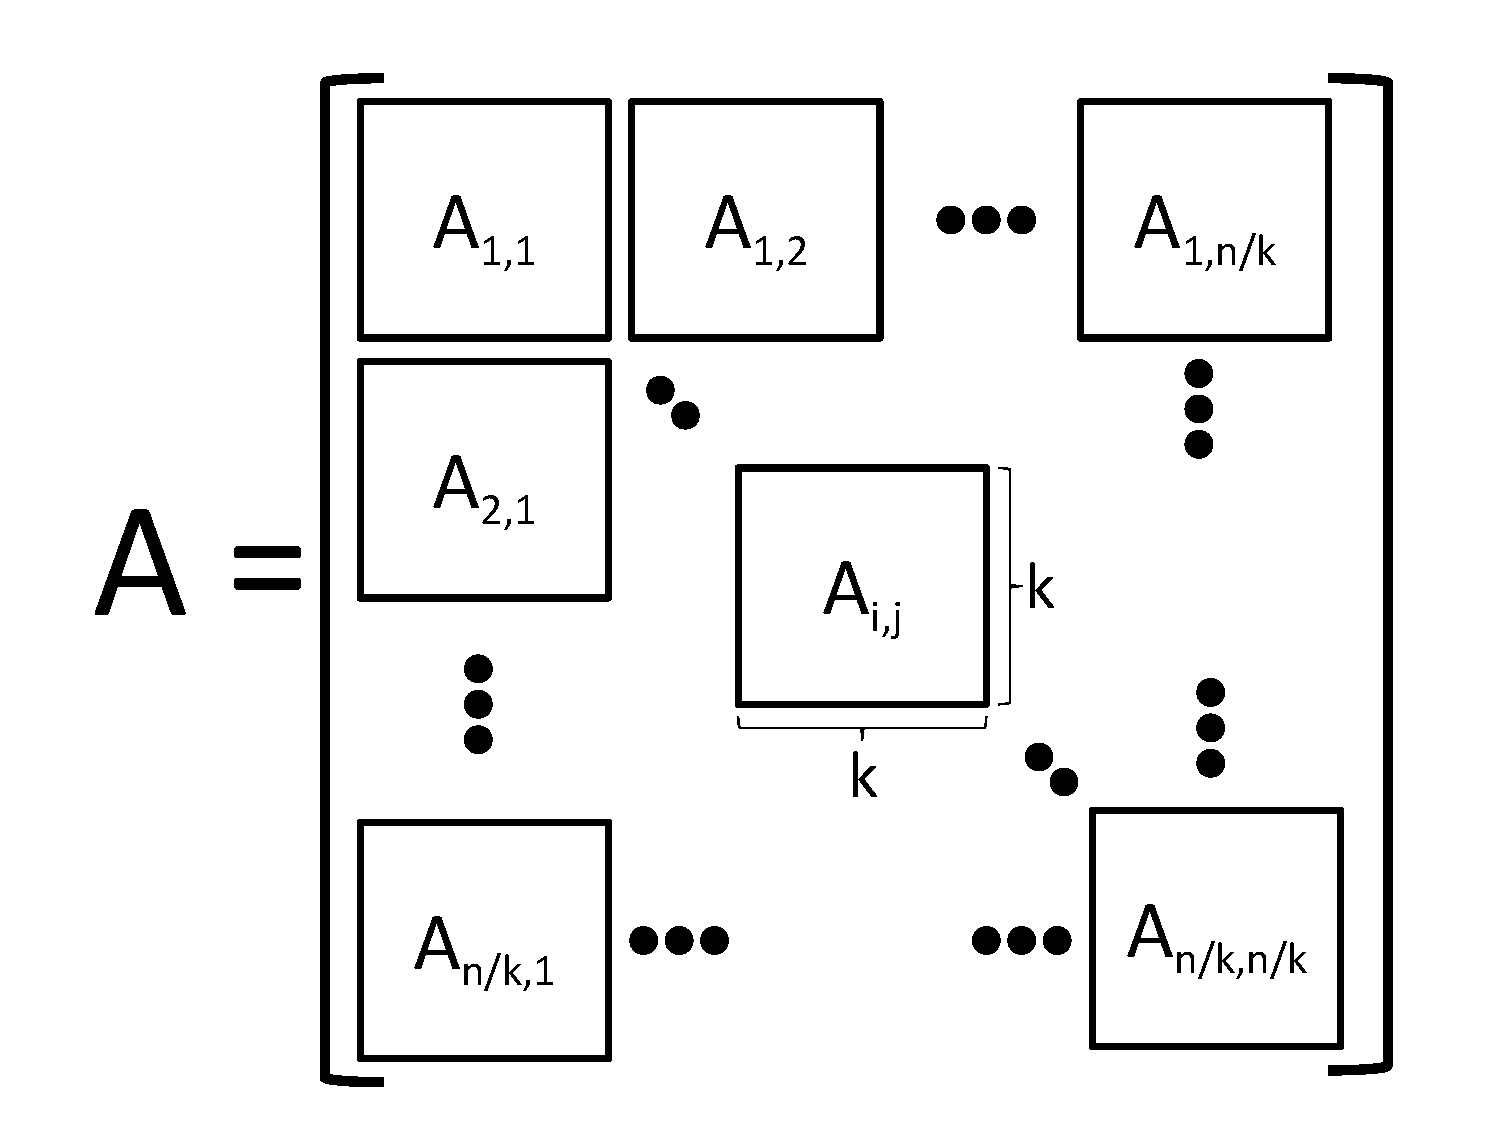
\includegraphics[scale=1, width=6cm]{figs/Pre-processing.pdf}
	}
\subfloat[][Structure of $LUT_i$]
	{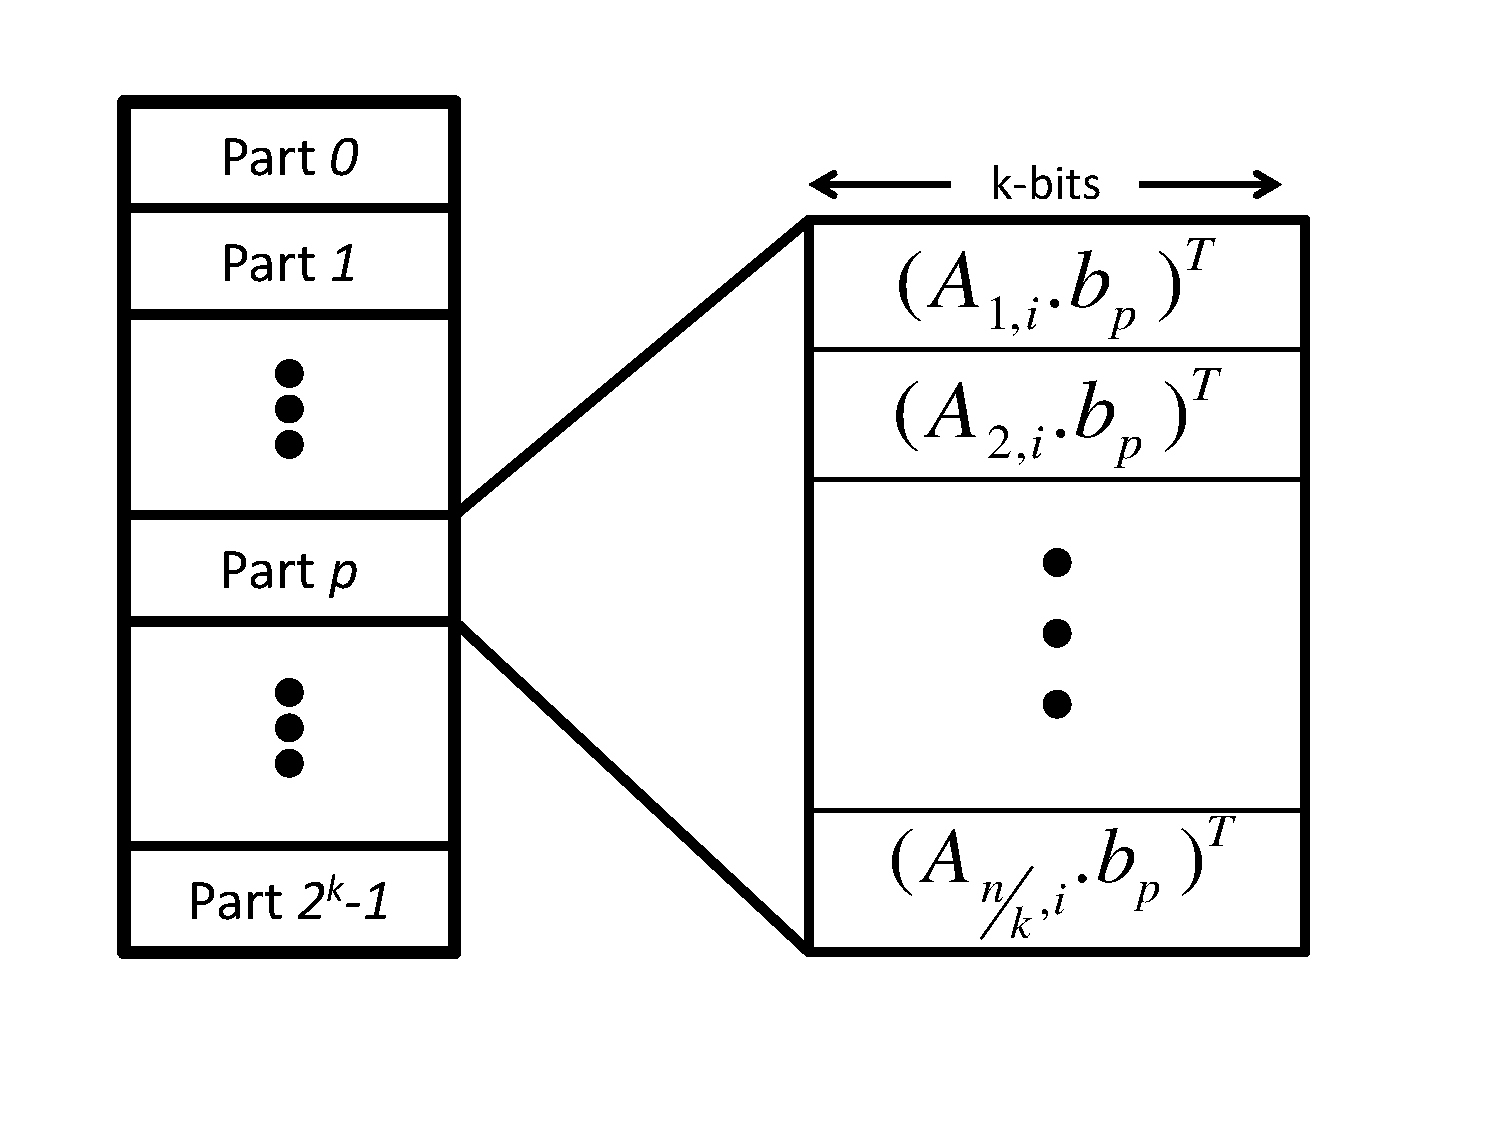
\includegraphics[scale=1, width=6cm]{figs/LUT.pdf}
	}
\caption{Preprocessing of Matrix $A$}	
\label{pre-process}
\end{figure*}

\subsubsection{Pre-processing Phase}
\begin{enumerate}

    \item Partition the input matrix \emph{A} into blocks (tiles) of size \emph{k} x \emph{k} bits
    as shown in Figure~\ref{pre-process}, for a given user defined parameter \emph{k}. The value of
this parameter \emph{k} has important ramifications on the requirements of the number of look-up
tables and computing nodes, size of the look-up tables and the number of operations during
pre-processing and computation phases. These relations would become clear by the end of this
section.  
  \item Construct $n/k$ loop-up tables (LUTs), labelled as $LUT_{1}, LUT_{2}, ..., LUT_{n/k}$, each
      of which further consists of $2^{k}$ partitions. These partitions are indexed from $0$ to
      $2^{k}-1$. Each partition consists of $n/k$ words of size $k$ bits.
  \item Populate the LUTs such that the $p$-th partition of $LUT_{i}$ consists of $k$-bit words
      corresponding to values $A_{1,i}.b_{p}, A_{2,i}.b_{p}, ... , A_{n/k,i}.b_{p}$. Here $b_{p}$ is
      a $k$-bit vector representation corresponding to the decimal value $p$. This means that $b_0$
      is an \emph{all-zero} vector and $b_{2^k-1}$ is an \emph{all-one} vector. The structure of the
      $LUT_i$ is also shown in Figure~\ref{pre-process}.
\end{enumerate}

Note that pre-processing step is equivalent to pre-computing and storing all possible products of
the blocks of matrix $A$, i.e. for $A_{1,1}, A_{1,2} .. A_{n/k,n/k}$. Since there are $2^{k}$ such
possible products for each block, and $n^{2}/k^{2}$ blocks, a total of $2^{k}.(n^{2}/k^{2})$ matrix
products are required during pre-processing. Since each of this product requires $O(k^{2})$
computational operations, and hence, the total pre-processing can be achieved in $O(n^{2}.2^{k})$
operations. Also if the vector $v$ and the product vector $v' = A.v$ are also partitioned into $n/k$
sub-vectors, each of size $k$-bits, as $v$ = $\begin{pmatrix} v_1 \\
    v_2 \\
    \vdots \\
    v_{n/k}
\end{pmatrix}$ and $v'$ = $\begin{pmatrix}
    v'_1 \\
    v'_2 \\
    \vdots \\
    v'_{n/k}
\end{pmatrix}$, then the sub-vector $v'_{i}$ can also be expressed as:

\begin{equation}~\label{BMVM:product}
	v'_{i} = (A_{i,1}.v_1) \vee (A_{i,2}.v_2) \vee ... (A_{i,n/k}.v_{n/k}) 
\end{equation}

In equation~\ref{BMVM:product}, the operator $\vee$ performs bit-wise \emph{xor}-operation on the
$k$-bit partial products. This is the essence of the computing phase described next.\\

\subsubsection{Computing Phase}

\begin{enumerate}
	\item Partition the input vector $v$ into $n/k$ $k$-bit sub-vectors $v_1, v_2, .. , v_{n/k}$, s.t. $v$ = $\begin{pmatrix}
    v_1 \\
    v_2 \\
    \vdots \\
    v_{n/k}
\end{pmatrix}$. Let $v'$ be another $n$-bit vector. Partition $v'$ into $k$-bit sub-vectors in a similar manner, as $v'$ = $\begin{pmatrix}
    v'_1 \\
    v'_2 \\
    \vdots \\
    v'_{n/k}
\end{pmatrix}$, and initialize it to $0$. 
    \item Look-up the partition $p_i$ in the look-up table $LUT_i$ (obtained from pre-processing)
    corresponding to the sub-vector $v_i$ for all $i$ in $\{1, 2, .., n/k\}$.  
    \item For the $j$-th
        ($j$ ranging from $1$ to $n/k$) word $e_j$ in partition $p_i$, update $v'_j$ as bit-wise
        $xor$ of current $v'_j$ with $e_j$. Do this for all partitions $p_i$, obtained in step 2.
%	\item To each of the $n/k$ $LUTs$ obtained from pre-processing, associate a computing node. Assume that these nodes can communicate with each other using $k$-bit messages and these nodes are indexed from $1$ to $n/k$. A compute node $i$ also maintains a $k$-bit register $v'_i$, initialized to $0$.
%	\item Partition the input vector $v$ into $n/k$ $k$-bit sub-vectors $v_1, v_2, .. , v_{n/k}$, s.t. $v$ = $\begin{pmatrix}
%    v_1 \\
%    v_2 \\
%    \vdots \\
%    v_{n/k}
%\end{pmatrix}$. 
%	\item A compute node indexed $i$ would look-up the partition $p_i$ in the look-up table $LUT_i$ corresponding to the sub-vector $v_i$. The compute node $i$ sends $(n/k)$ $k$-bit values in the partition $p_i$ to the corresponding compute nodes (one of these $n/k$ messages is sent to itself). 
%	\item Every compute node would receive $n/k$ such $k$-bit messages. The register $v'_i$ corresponding to node $i$ is computed by bit-wise $xor$ of all the messages received by node $i$. This is also shown in Figure~\ref{•}.
	\item The product $A.v$ is then given by $v'$ = $\begin{pmatrix}
    v'_1 \\
    v'_2 \\
    \vdots \\
    v'_{n/k}
\end{pmatrix}$. 
\end{enumerate}

It can be inferred easily that the computing phase requires $n^2/k^2$ bit-wise $xor$-operations of
size $k$-bits. The matrix-vector multiplication can, therefore, be computed in $O(n^2/k^2)$.
In~\cite{williams2007matrix}, the authors have used $k = \epsilon log_2(n)$, with $\epsilon < 0.5$,
so that the multiplication can be carried out in $O(n^2/(\epsilon log(n))^2)$ on a $log(n)$-word
RAM. 

We summarize the important analysis related to the algorithm, when used with parameter $k$ here:\\
Word width of LUT = $k$ \\
Number of LUTs = $n/k$ \\
Size of each LUT (in words) = $2^k.(n/k)$ \\
Number of word operations required = $n^2/k^2$ \\

It is observable that increasing the value of $k$ would reduce the computation time due to the
reduced number of operations, but would, in turn, also increase the memory requirement (in LUTs) and
the pre-processing time (occurring in $O(2^k.(n^2/k^2))$ ) exponentially. A careful selection of the
parameter $k$ is thus required for achieving the right balance between the three. Also note that the
extreme case when $k = n$ requires a single LUT storing $n$-bit product vectors corresponding to all
possible $2^n$ combinations of input vector. Any multiplication would only require a single look-up
into the corresponding entry. However, this is exponential in memory and pre-processing time and
cannot be applied to matrices exceeding a few 10s of bits in size.

\subsection{Implementation Details}~\label{sec:Impl}

%software - pre-processing
%
%memory - > Distributed BRAM structure in FPGA. initialization
%compute node
%Why NoC - simplified communication between nodes. scalable. also can be easily partitioned over multiple fpgas. helps meet timing constraints.
%no synchronization. one packet per cycle
%folding - advantage - smaller topology can be used. increases network utilization. also mention about broadcast.
%
%software- multi-threaded. synchronization. folding. possibility of optimization

%Part1~\cite{KandR} has~\cite{taylor2012dark,uba,ipek2007,ibmp5}

In this section, we shall describe the implementation details of the algorithm described in Section~\ref{sec:BMVM}. The goal of our implementation is to have a \emph{flexible} and \emph{scalable} software library framework for FPGA-accelerated iterative boolean matrix multiplication using the above algorithm.\\

\subsubsection{Pre-processing}

As described in section~\ref{sec:BMVM}, the algorithm is composed of two phases: the pre-processing phase and the computation phase. Since the pre-processing phase is required only once for a given input matrix, which is assumed to be re-used multiple times over several iterations in the target applications, we apply this phase completely on the software end using MATLAB. The entire source code, along with usage details, for this step in available in section~\ref{appendix}. The script takes the matrix size $n$, $\epsilon$(s.t. $k = \epsilon .log(n)$) and folding factor as an input parameter. We describe the concept of "folding", which is used by the folding factor, later in this section.\\

It must the noted that although the authors in~\cite{williams2007matrix} use $\epsilon < 0.5$ for reasons mentioned already, we make no such assumption and leave it to the user to best determine the appropriate value of $\epsilon$. The code produces several '.txt' and '.data' files as output, corresponding to the look-up tables used in the FPGA and software implementation of the algorithm, respectively and having the same structure as described in Figure~\ref{pre-process}(b). The $LUTs$ are generated by multiplying each blocks (tiles) of size $k$x$k$ of the input matrix $A$ by all possible vector combinations of size $k$, and storing the output values. In the current code, the matrix $A$, of size $n$x$n$, is randomly generated with uniform probability of $1's$ and $0's$. The matrix size if also assumed to be a power of 2, which can be easily modified to make it more general.\\

\subsubsection{Hardware implementation}

We now start discussing the FPGA implementation of the algorithm. As evident in section!\ref{sec:BMVM}, the algorithm is memory-intensive, rather than computation-intensive, due to the large sizes of the look-up-tables. To preserve data locality and improve computation time, we would like the $LUTs$ to completely reside on the FPGA hardware. In order to best utilize the available memory resources in the FPGA, we first observe that modern FPGAs are provisioned with abundant Block RAM (BRAM) resources. For instance, \emph{Xilinx Vitex 6} (used in this work) has a large number of 36Kb Block RAMs, totalling upto 38Mb of internal BRAM storage. The internal structure of a typical FPGA is shown in Figure~\ref{FPGA}. It can be observed that the Block RAMs are broadly distributed over the entire FPGA fabric.\\

\begin{figure}[t!]
\centering
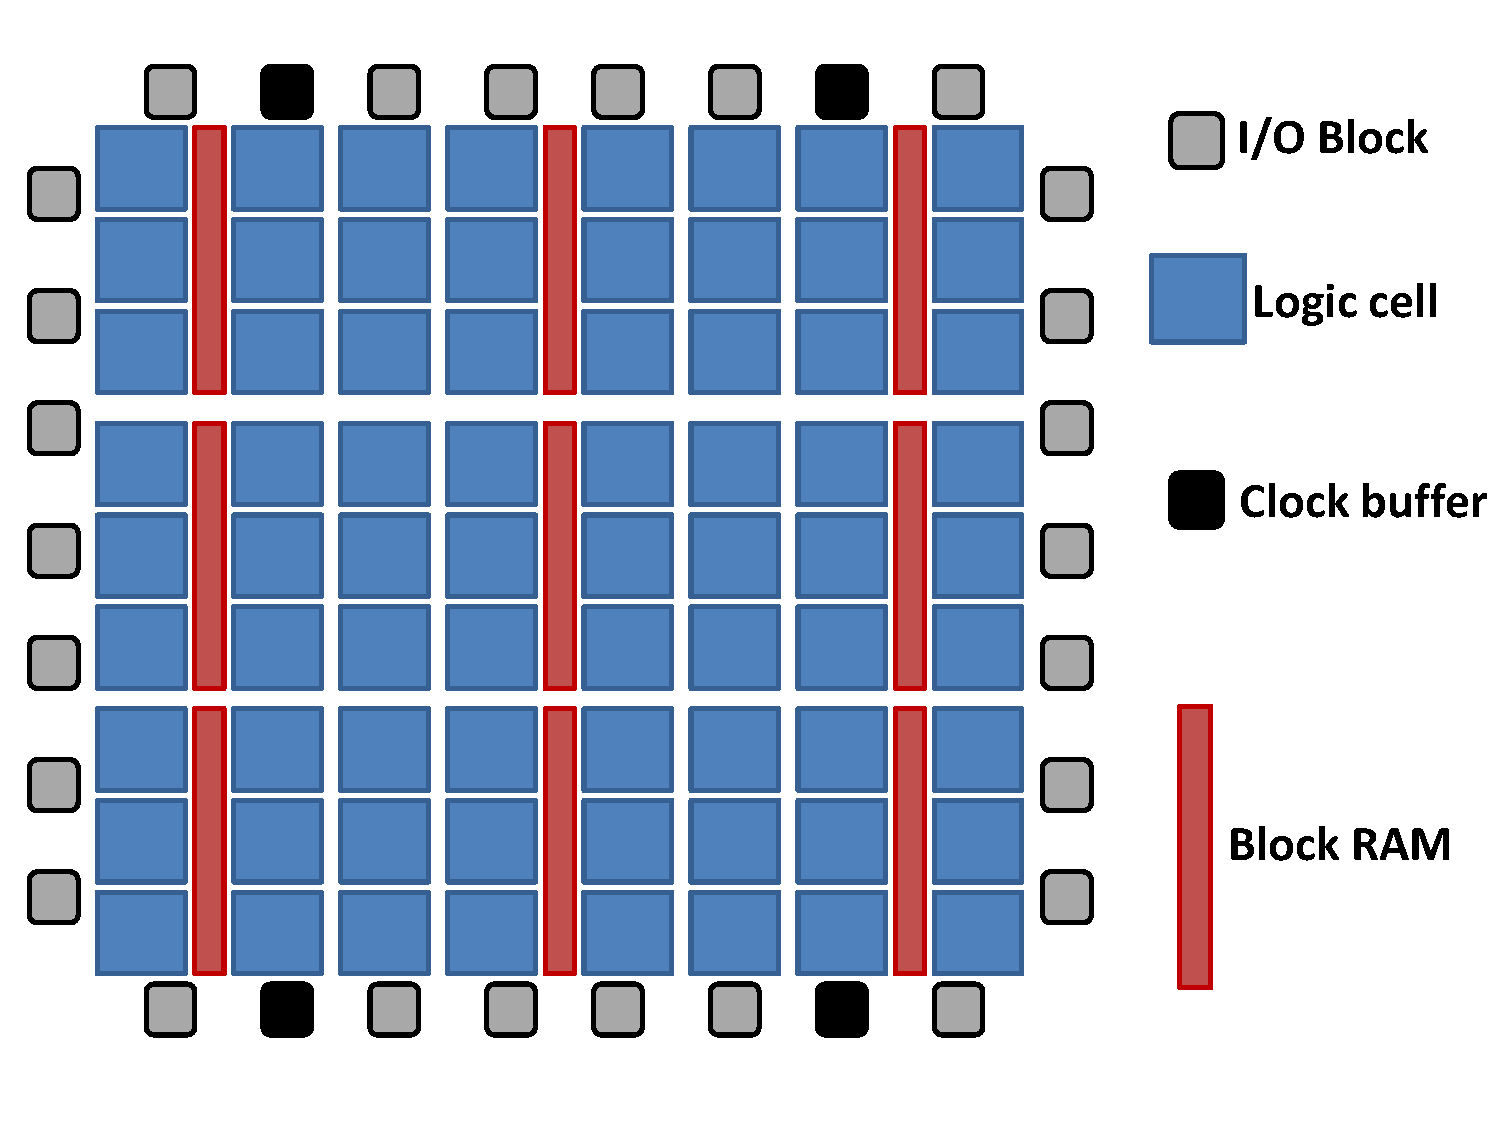
\includegraphics[scale=1, width=8cm]{figs/FPGA.pdf}
\caption{FPGA internal structure.}
\label{FPGA}
\end{figure}

As mentioned earlier, the memory requirement of a single $LUT$ is $(n/k)*2^k$ words (with each word storing $k$ bits). We would ideally like the $LUTs$ to be implemented automatically using Block RAMs. 
% In order to achieve this, we use the following template for an $LUT$:
% 
% \begin{lstlisting}[label=LUT, language=Verilog]
%  module LUT( clk, write_enable, address, input_data, output_data);
%  .
%  .
%  .  
%    parameter file_name = "preprocessed_1.data";
%    reg [RAM_WIDTH-1:0] RAM_1R1W [(2**RAM_ADDR_BITS)-1:0];
%  
%    initial
%       $readmemb(file_name, RAM_1R1W , 0, (2**RAM_ADDR_BITS)-1);
% 	  
%    always @(posedge clk) begin
%    output_data <= RAM_1R1W[address];
%          if (write_enable)
%            RAM_1R1W[address] <= input_data;
%    end
%  .
%  .
%  .
%  endmodule 
% \end{lstlisting}
% This allows the (Xilinx) synthesiser tool to automatically infer Block RAMs for the $LUTs$. Also note that the code uses \emph{\$readmeb} command to read and initialize the $LUTs$ directly from the pre-processed input files (provided using parameter in this module), so that the initialization is not required.  \\
  
It must be noted that the loop-up tables, implemented in the form of Block RAMs are required to ``exchange information" based the algorithm described in Section~\ref{sec:BMVM}. The BRAMs could be situated far off from each other on an FPGA, or even reside on different FPGAs altogether, in a multi-FPGA implementation (memory constraint of FPGA limits the size and number of LUTs that can reside on a single FPGA). Network-on-chip would not only help in seamless communication between the LUTs, but would also help improve the clock speed. In our FPGA implementation, with each of the $n/k$ $LUTs$ obtained from pre-processing, we associate a ``computing node". These nodes can communicate with each other using $k$-bit messages over an NoC and these nodes are indexed from $1$ to $n/k$. A compute node $i$ also maintains a $k$-bit register $v'_i$, initialized to $0$. A compute node indexed $i$ would look-up the partition $p_i$ in the look-up table $LUT_i$ corresponding to the sub-vector $v_i$. The compute node $i$ 
sends $(n/k)$ $k$-bit values in the partition $p_i$ to the corresponding compute nodes. Every compute node also would receive $n/k$ such $k$-bit messages. The register $v'_i$ corresponding to node $i$ is computed by bit-wise $xor$ of all the messages received by node $i$. The product $A.v$ is then given by $v'$ = $\begin{pmatrix}
    v'_1 \\
    v'_2 \\
    \vdots \\
    v'_{n/k}
\end{pmatrix}$. \\
%	\item Partition the input vector $v$ into $n/k$ $k$-bit sub-vectors $v_1, v_2, .. , v_{n/k}$, s.t. $v$ = $\begin{pmatrix}
%    v_1 \\
%    v_2 \\
%    \vdots \\
%    v_{n/k}
%\end{pmatrix}$.  

%% synchronization
% folding
% iterative
% parameters
% FSM
% hierarchy
% RIFFA

We use a NoC generated by CONNECT\cite{papamichael2012connect} for our implementation in which the computing nodes are connected as the ``processing elements" (PEs) at the input/output ports of the generated NoC. These nodes use the interface provided by CONNECT to exchange messages. It is important to ensure that while multiple such messages may simultaneously attempt to update a particular product sub-vector $v'_i$, the updates are appropriately serialized to maintain correctness. Since only one flit can be injected and ejected in a single cycle in the NoC, this constraint is automatically ensured. our implementation supports the following ``Network and Router Options" for NoC generated using CONNECT (topology and number of endpoints is user-specified):
\begin{itemize}
	\item \textbf{Router Type:} Simple Input Queued (IQ)
	\item \textbf{Flow Control Type:} Peek Flow Control
	\item \textbf{Flit Data Width:} 16
	\item \textbf{Flit Buffer Depth:} 8
	\item \textbf{Allocator:} Separable Input first Round-Robin
\end{itemize}


\begin{figure}[t!]
\centering
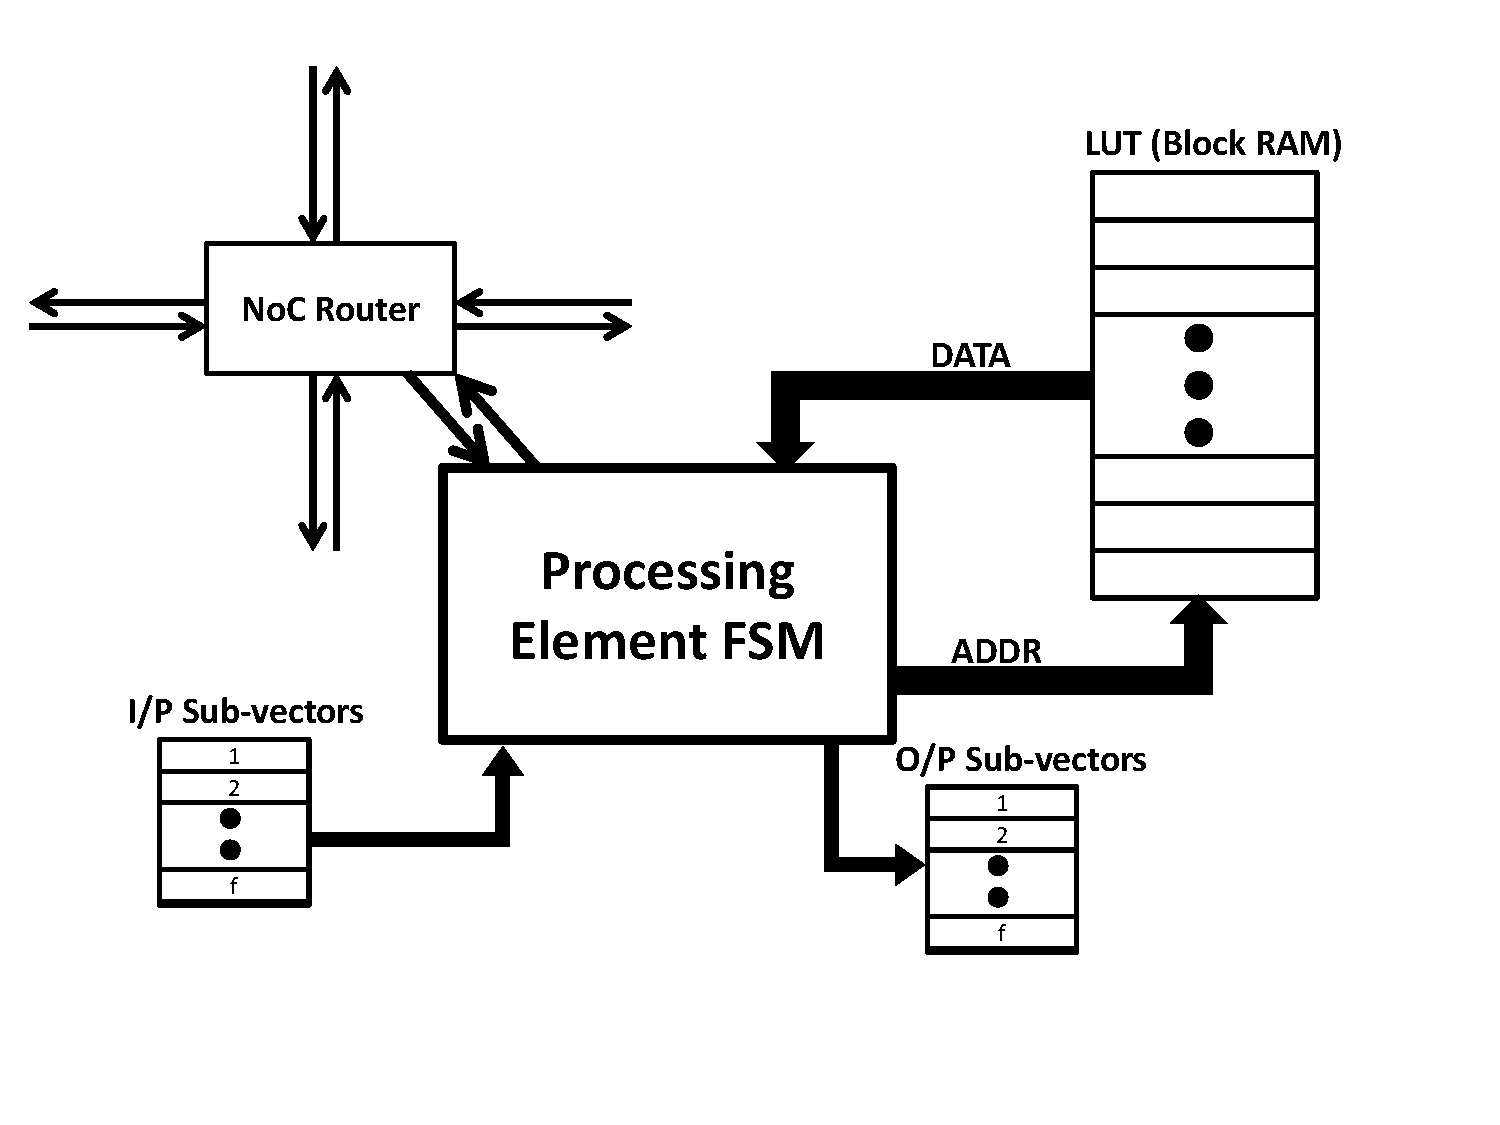
\includegraphics[scale=1, width=10cm]{figs/processing_element.pdf}
\caption{Processing element.}
\label{fig:pe}
\end{figure}

Since the number of computing nodes required grows linearly with the matrix size (as $n/k$), the number of ports required for the NoC would also grow linearly. This could pose and exorbitant requirement on the number of NoC ports since most topologies do not scale well to a very large number of endpoints. To this end, we implement ``folding" of computing nodes,  which allows multiple processing elements connected to a single endpoint of an NoC to serve as multiple computing nodes. The extent of such folding, referred to as the ``folding factor" $f$, is a user-specified parameter in our implementation. Our folding follows a cyclic assignment, i.e. an instance with $n$ computing nodes and $n/f$ processing elements or endpoints, would assign computing nodes $1, f+1, 2f+1, ..., (n-f) + 1$ computing nodes to the processing element $1$. Since a single processing element is now required to send and receive $f^2$ times the number of messages to the case where there is no folding with same number of processing 
elements (or ports in the network), the message traffic would also increase, resulting in higher network utilization. Since only one message can be sent/received on a single NoC port, the folded design would exploit lower concurrency, thereby lowering performance. The folding parameter is also specified while generating the LUTs in the pre-processing step, which results in large memory sizes compared to the case of no folding. The caveat of large folding, however, is that large LUT could also lower the maximum operational frequency of the design, thereby further lowering its overall performance. These effects are discussed in greater detail in Chapter~\ref{C:Exp}. Figure~\ref{fig:pe} shows a single processing element (multiplication node) with folding factor $f$ in our implementation. \\

Since a number of our target applications require computation of several iterations of boolean vector multiplications, \emph{viz.} $A.v, A^2.v, ..., A^k.v$, given an input vector $v$, we provision our processing elements to support iterative matrix vector product. The number of such iterations is again provided as parameter by the user. Support for iterative multiplication would require the processing elements to perform multiplication of matrix $A$ with input vector $v'_k$ in the $kth$ iteration, where $v'_k$ is the resulting product vector after the $(k-1)th$ iteration. Since the resulting sub-vectors $v'_k$ are local to the processing elements in the $kth$ iteration, this task seems trivial. However, iterative multiplication poses a unique challenge of $synchronization$ of processing nodes after every iteration. This means that a processing element should only commence the $k$th iteration after ensuring that all other processing elements are also ready for starting $k$th iteration. If this is not the case 
and a processing element (which has already sent and received all messages of previous iteration) jumps to next iteration before others, the messages sent by this PE could be misinterpreted by other PEs to belong to previous iteration, resulting in incorrect computation of product values. One solution could be to use additional bits in messages to indicate the $id$ for the iteration to which the message belongs. This would allow PEs to proceed to next iteration without waiting for others but this is expensive as the flit width is limited and this would also require buffering of incoming messages of future iterations. Other option could also be to use special messages to broadcast information to all PEs whenever a PE has completed an iteration. Each PE would maintain a list of completed PEs and would proceed to next iteration only after ensuring all others are also ready to proceed. While this seems more feasible, it also has performance penalty associated with the broadcast messages after every iteration.\\

\begin{figure}[t!]
\centering
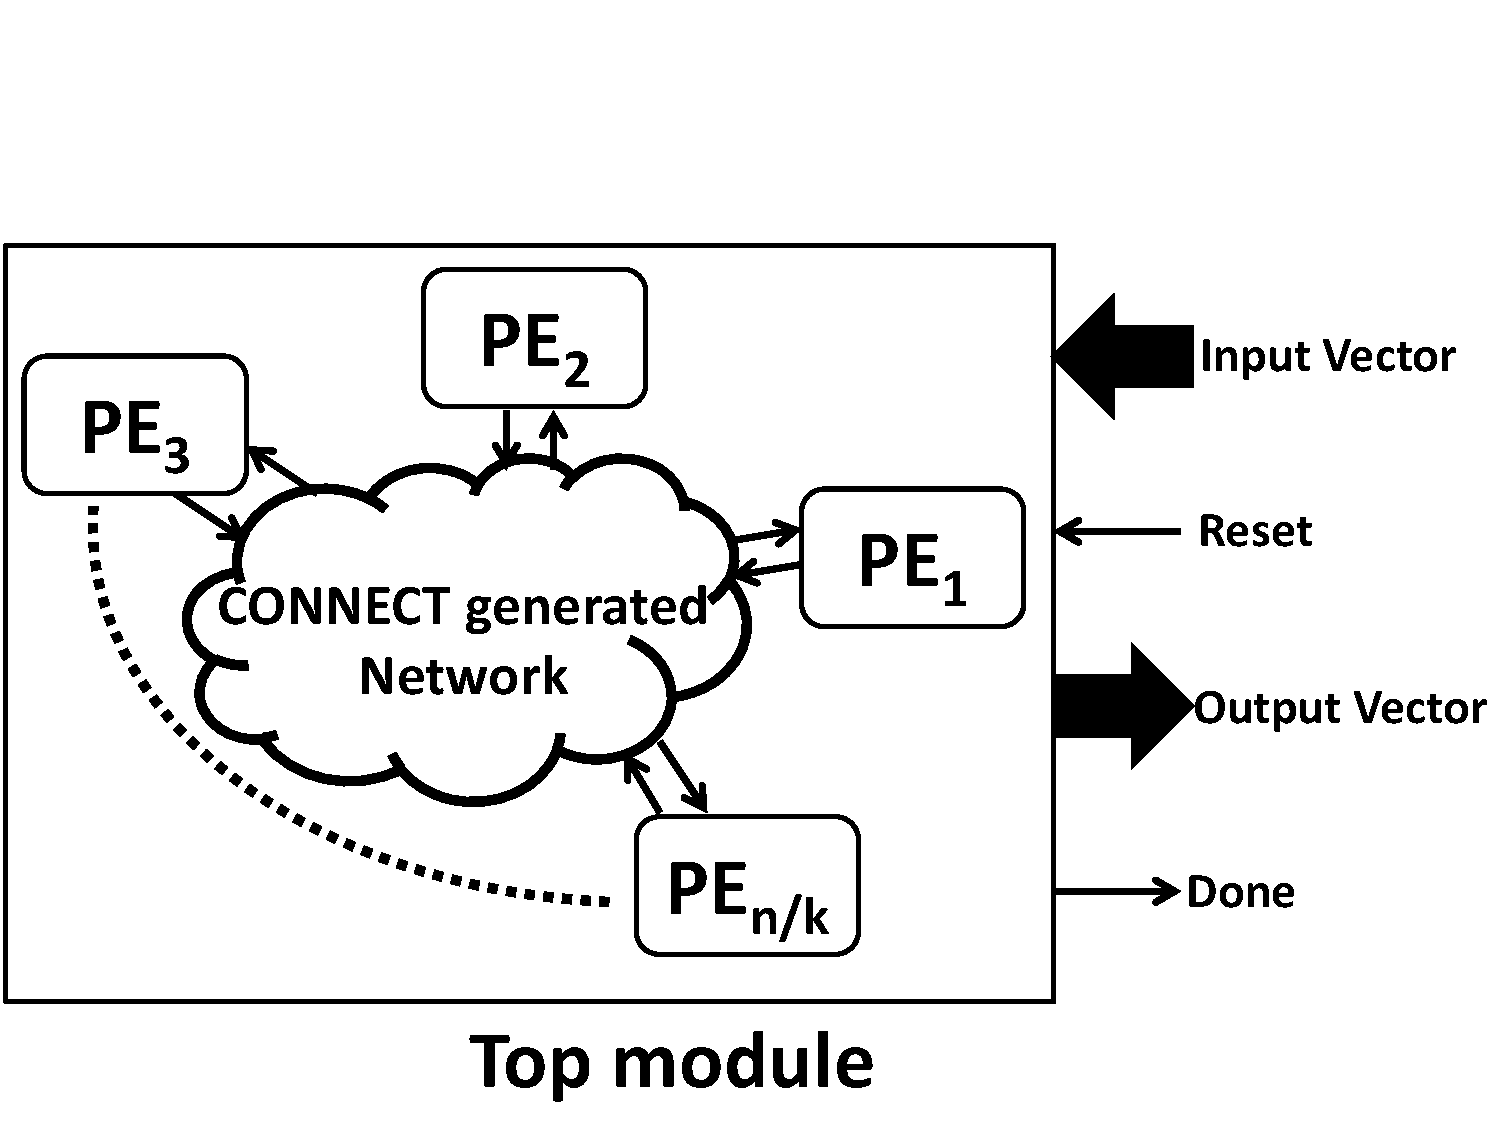
\includegraphics[scale=1, width=10cm]{figs/mult_top.pdf}
\caption{Top module for Boolean Matrix Vector Multiplication (BMVM).}
\label{fig:mult_top}
\end{figure}

In our approach, we observe that the behaviour of the network after in each iteration would be exactly identical if the PEs are exactly synchronized. Therefore, if we know the maximum number of cycles required for a PE to complete an iteration, all PEs could wait to synchronize at this cycle count after every iteration, thereby eliminating the need for additional broadcast messages. It is important to note that this count is dependent on the topology and routing policy used. We specify the count as a parameter to the processing element in our design, which could be determined by the user by simulating one iteration of the multiplication on the software. Our processing elements display the cycle counts at which the processing elements are done with one iteration (when they have sent and received all messages pertaining to that iteration), and the maximum of this count can be specified in that parameter. The source code of our processing element is included in~\ref{•}. Other parameters used by this module are 
specified and explained in~\ref{•}. Figure~\ref{fig:mult_top} shows the top level user module along with their module names in our design, consisting of several instances of processing elements connected by a CONNECT generated NoC. It must be noted that the NoC can itself be partitioned using our script, in which case the top module would consist of multiple instances for NoC corresponding to different partitions, with serial wire and flow control signals between them. We have only tested our partitioned NoC for boolean vector multiplication on a single FPGA, with wires corresponding to different partitions connected internally. Since the partitioned NoC itself has been tested successfully on separate Virtex 5 boards, we believe that multiplier design should also work for multi-FPGA case. The interface to the top module is kept as simple as providing the input vector followed by a reset signal as input, and obtaining the output vector on the done signal at the output.\\

In our final step, we wish to encapsulate our multiplication hardware within a software library to make it usable for target applications, mostly running on software. For this purpose, we use Reusable Integration Framework for FPGA Accelerators (RIFFA 2.0)~\cite{jacobsen2013riffa}, which provides a simple open-source integration framework for FPGA-CPU communication over high-speed PCIe links. On the software end, RIFFA provides a simple API to open/close an FPGA connection, send/receive data from FPGA and to send reset the FPGA user module. Although we use a single channel (corresponding to network sockets and parallel user cores), RIFFA can support upto 12 channels. The data transfers in RIFFA occur through PCIe transactions, with FPGA acting as the DMA bus master. For more details, the reader can refer to~\cite{jacobsen2013riffa}. \\

\begin{figure}[t!]
\centering
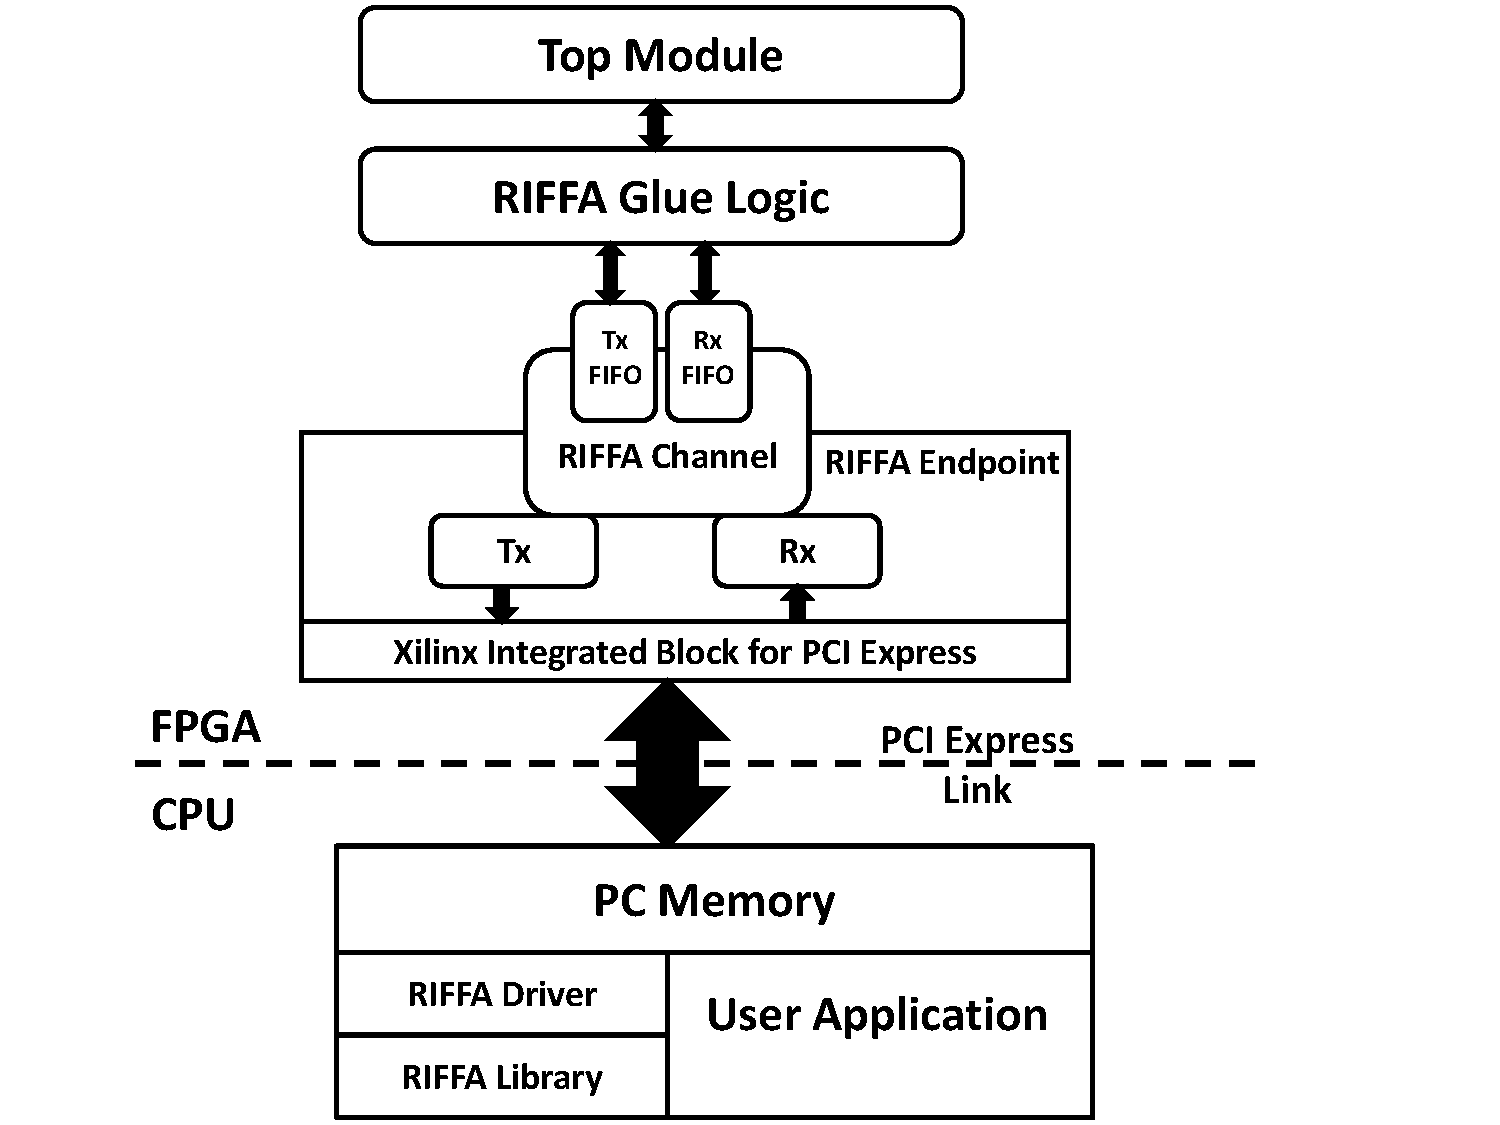
\includegraphics[scale=0.20]{figs/riffa.pdf}
\caption{BMVM framework with RIFFAa.}
\label{fig:riffa}
\end{figure}

We demonstrate the usage using a simple C application shown in ~\ref{•}. The application resets the FPGA and sends an input vector, on which the multiplication is performed by the FPGA, before waiting to receive the output product. Since the application is written for a 32-bit processor, appropriate precautions are taken to make it compatible with the \emph{little endianess} of the RIFFA hardware modules supporting 64-bits. We also implement the necessary glue logic for the hardware interface between RIFFA endpoint and multiplier module as shown in Figure~\ref{fig:riffa}. The code for this module is available in ~\ref{•}.\\  
      
\section{Implementation Details}~\label{sec:Impl}

%software - pre-processing
%
%memory - > Distributed BRAM structure in FPGA. initialization
%compute node
%Why NoC - simplified communication between nodes. scalable. also can be easily partitioned over multiple fpgas. helps meet timing constraints.
%no synchronization. one packet per cycle
%folding - advantage - smaller topology can be used. increases network utilization. also mention about broadcast.
%
%software- multi-threaded. synchronization. folding. possibility of optimization

%Part1~\cite{KandR} has~\cite{taylor2012dark,uba,ipek2007,ibmp5}

In this section, we shall describe the implementation details of the algorithm described in Section~\ref{sec:BMVM}. The goal of our implementation is to have a \emph{flexible} and \emph{scalable} software library framework for FPGA-accelerated iterative boolean matrix multiplication using the above algorithm.\\

\subsection{Pre-processing}

As described in section~\ref{sec:BMVM}, the algorithm is composed of two phases: the pre-processing phase and the computation phase. Since the pre-processing phase is required only once for a given input matrix, which is assumed to be re-used multiple times over several iterations in the target applications, we apply this phase completely on the software end using MATLAB. The entire source code, along with usage details, for this step in available in section~\ref{appendix}. The script takes the matrix size $n$, $\epsilon$(s.t. $k = \epsilon .log(n)$) and folding factor as an input parameter. We describe the concept of "folding", which is used by the folding factor, later in this section.\\

It must the noted that although the authors in~\cite{williams2007matrix} use $\epsilon < 0.5$ for reasons mentioned already, we make no such assumption and leave it to the user to best determine the appropriate value of $\epsilon$. The code produces several '.txt' and '.data' files as output, corresponding to the look-up tables used in the FPGA and software implementation of the algorithm, respectively and having the same structure as described in Figure~\ref{pre-process}(b). The $LUTs$ are generated by multiplying each blocks (tiles) of size $k$x$k$ of the input matrix $A$ by all possible vector combinations of size $k$, and storing the output values. In the current code, the matrix $A$, of size $n$x$n$, is randomly generated with uniform probability of $1's$ and $0's$. The matrix size if also assumed to be a power of 2, which can be easily modified to make it more general.\\

\subsection{Hardware implementation}

We now start discussing the FPGA implementation of the algorithm. As evident in section!\ref{sec:BMVM}, the algorithm is memory-intensive, rather than computation-intensive, due to the large sizes of the look-up-tables. To preserve data locality and improve computation time, we would like the $LUTs$ to completely reside on the FPGA hardware. In order to best utilize the available memory resources in the FPGA, we first observe that modern FPGAs are provisioned with abundant Block RAM (BRAM) resources. For instance, \emph{Xilinx Vitex 6} (used in this work) has a large number of 36Kb Block RAMs, totalling upto 38Mb of internal BRAM storage. The internal structure of a typical FPGA is shown in Figure~\ref{FPGA}. It can be observed that the Block RAMs are broadly distributed over the entire FPGA fabric.\\

\begin{figure}[t!]
\centering
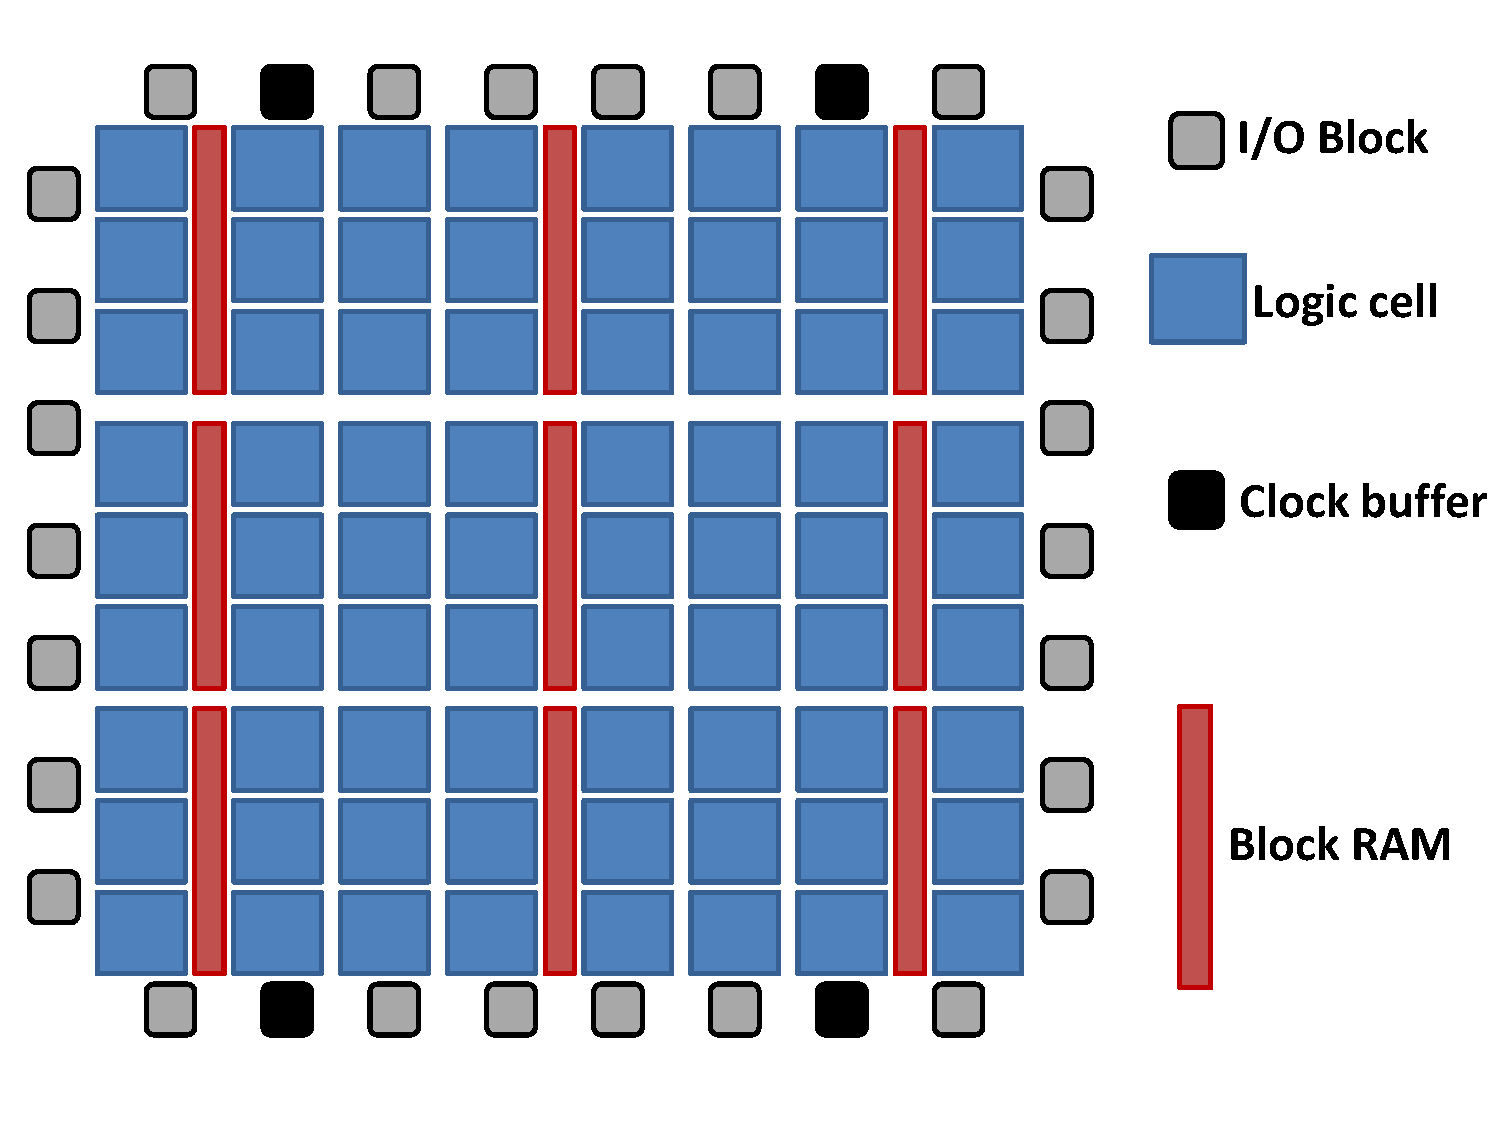
\includegraphics[scale=0.35]{figs/FPGA.pdf}
\caption{FPGA internal structure.}
\label{FPGA}
\end{figure}

% As mentioned earlier, the memory requirement of a single $LUT$ is $(n/k)*2^k$ words (with each word storing $k$ bits). We would ideally like the $LUTs$ to be implemented automatically using Block RAMs. In order to achieve this, we use the following template for an $LUT$:
% 
% \begin{lstlisting}[label=LUT, language=Verilog]
%  module LUT( clk, write_enable, address, input_data, output_data);
%  .
%  .
%  .  
%    parameter file_name = "preprocessed_1.data";
%    reg [RAM_WIDTH-1:0] RAM_1R1W [(2**RAM_ADDR_BITS)-1:0];
%  
%    initial
%       $readmemb(file_name, RAM_1R1W , 0, (2**RAM_ADDR_BITS)-1);
% 	  
%    always @(posedge clk) begin
%    output_data <= RAM_1R1W[address];
%          if (write_enable)
%            RAM_1R1W[address] <= input_data;
%    end
%  .
%  .
%  .
%  endmodule 
% \end{lstlisting}
% This allows the (Xilinx) synthesiser tool to automatically infer Block RAMs for the $LUTs$. Also note that the code uses \emph{\$readmeb} command to read and initialize the $LUTs$ directly from the pre-processed input files (provided using parameter in this module), so that the initialization is not required.  \\
  
It must be noted that the loop-up tables, implemented in the form of Block RAMs are required to ``exchange information" based the algorithm described in Section~\ref{sec:BMVM}. The BRAMs could be situated far off from each other on an FPGA, or even reside on different FPGAs altogether, in a multi-FPGA implementation (memory constraint of FPGA limits the size and number of LUTs that can reside on a single FPGA). Network-on-chip would not only help in seamless communication between the LUTs, but would also help improve the clock speed. In our FPGA implementation, with each of the $n/k$ $LUTs$ obtained from pre-processing, we associate a ``computing node". These nodes can communicate with each other using $k$-bit messages over an NoC and these nodes are indexed from $1$ to $n/k$. A compute node $i$ also maintains a $k$-bit register $v'_i$, initialized to $0$. A compute node indexed $i$ would look-up the partition $p_i$ in the look-up table $LUT_i$ corresponding to the sub-vector $v_i$. The compute node $i$ 
sends $(n/k)$ $k$-bit values in the partition $p_i$ to the corresponding compute nodes. Every compute node also would receive $n/k$ such $k$-bit messages. The register $v'_i$ corresponding to node $i$ is computed by bit-wise $xor$ of all the messages received by node $i$. The product $A.v$ is then given by $v'$ = $\begin{pmatrix}
    v'_1 \\
    v'_2 \\
    \vdots \\
    v'_{n/k}
\end{pmatrix}$. \\
%	\item Partition the input vector $v$ into $n/k$ $k$-bit sub-vectors $v_1, v_2, .. , v_{n/k}$, s.t. $v$ = $\begin{pmatrix}
%    v_1 \\
%    v_2 \\
%    \vdots \\
%    v_{n/k}
%\end{pmatrix}$.  

%% synchronization
% folding
% iterative
% parameters
% FSM
% hierarchy
% RIFFA

We use a NoC generated by CONNECT\cite{papamichael2012connect} for our implementation in which the computing nodes are connected as the ``processing elements" (PEs) at the input/output ports of the generated NoC. These nodes use the interface provided by CONNECT to exchange messages. It is important to ensure that while multiple such messages may simultaneously attempt to update a particular product sub-vector $v'_i$, the updates are appropriately serialized to maintain correctness. Since only one flit can be injected and ejected in a single cycle in the NoC, this constraint is automatically ensured. our implementation supports the following ``Network and Router Options" for NoC generated using CONNECT (topology and number of endpoints is user-specified):
\begin{itemize}
	\item \textbf{Router Type:} Simple Input Queued (IQ)
	\item \textbf{Flow Control Type:} Peek Flow Control
	\item \textbf{Flit Data Width:} 16
	\item \textbf{Flit Buffer Depth:} 8
	\item \textbf{Allocator:} Separable Input first Round-Robin
\end{itemize}


\begin{figure}[t!]
\centering
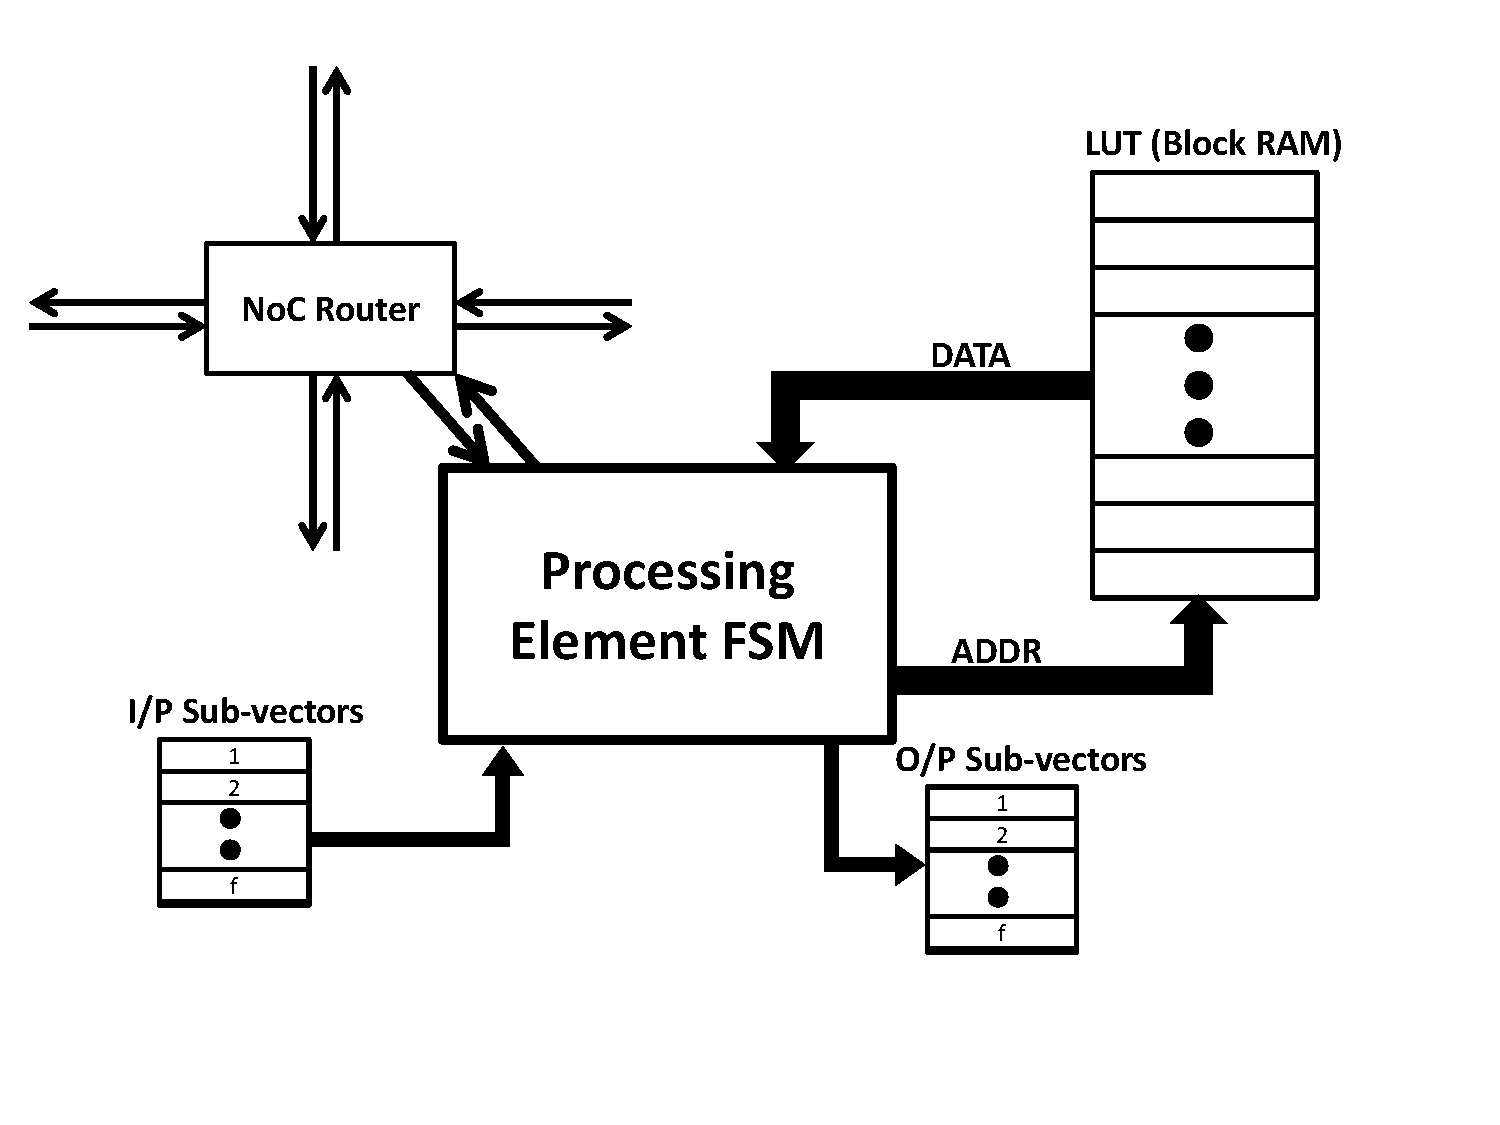
\includegraphics[scale=0.35]{figs/processing_element.pdf}
\caption{Processing element.}
\label{fig:pe}
\end{figure}

Since the number of computing nodes required grows linearly with the matrix size (as $n/k$), the number of ports required for the NoC would also grow linearly. This could pose and exorbitant requirement on the number of NoC ports since most topologies do not scale well to a very large number of endpoints. To this end, we implement ``folding" of computing nodes,  which allows multiple processing elements connected to a single endpoint of an NoC to serve as multiple computing nodes. The extent of such folding, referred to as the ``folding factor" $f$, is a user-specified parameter in our implementation. Our folding follows a cyclic assignment, i.e. an instance with $n$ computing nodes and $n/f$ processing elements or endpoints, would assign computing nodes $1, f+1, 2f+1, ..., (n-f) + 1$ computing nodes to the processing element $1$. Since a single processing element is now required to send and receive $f^2$ times the number of messages to the case where there is no folding with same number of processing 
elements (or ports in the network), the message traffic would also increase, resulting in higher network utilization. Since only one message can be sent/received on a single NoC port, the folded design would exploit lower concurrency, thereby lowering performance. The folding parameter is also specified while generating the LUTs in the pre-processing step, which results in large memory sizes compared to the case of no folding. The caveat of large folding, however, is that large LUT could also lower the maximum operational frequency of the design, thereby further lowering its overall performance. These effects are discussed in greater detail in Chapter~\ref{C:Exp}. Figure~\ref{fig:pe} shows a single processing element (multiplication node) with folding factor $f$ in our implementation. \\

Since a number of our target applications require computation of several iterations of boolean vector multiplications, \emph{viz.} $A.v, A^2.v, ..., A^k.v$, given an input vector $v$, we provision our processing elements to support iterative matrix vector product. The number of such iterations is again provided as parameter by the user. Support for iterative multiplication would require the processing elements to perform multiplication of matrix $A$ with input vector $v'_k$ in the $kth$ iteration, where $v'_k$ is the resulting product vector after the $(k-1)th$ iteration. Since the resulting sub-vectors $v'_k$ are local to the processing elements in the $kth$ iteration, this task seems trivial. However, iterative multiplication poses a unique challenge of $synchronization$ of processing nodes after every iteration. This means that a processing element should only commence the $k$th iteration after ensuring that all other processing elements are also ready for starting $k$th iteration. If this is not the case 
and a processing element (which has already sent and received all messages of previous iteration) jumps to next iteration before others, the messages sent by this PE could be misinterpreted by other PEs to belong to previous iteration, resulting in incorrect computation of product values. One solution could be to use additional bits in messages to indicate the $id$ for the iteration to which the message belongs. This would allow PEs to proceed to next iteration without waiting for others but this is expensive as the flit width is limited and this would also require buffering of incoming messages of future iterations. Other option could also be to use special messages to broadcast information to all PEs whenever a PE has completed an iteration. Each PE would maintain a list of completed PEs and would proceed to next iteration only after ensuring all others are also ready to proceed. While this seems more feasible, it also has performance penalty associated with the broadcast messages after every iteration.\\

\begin{figure}[t!]
\centering
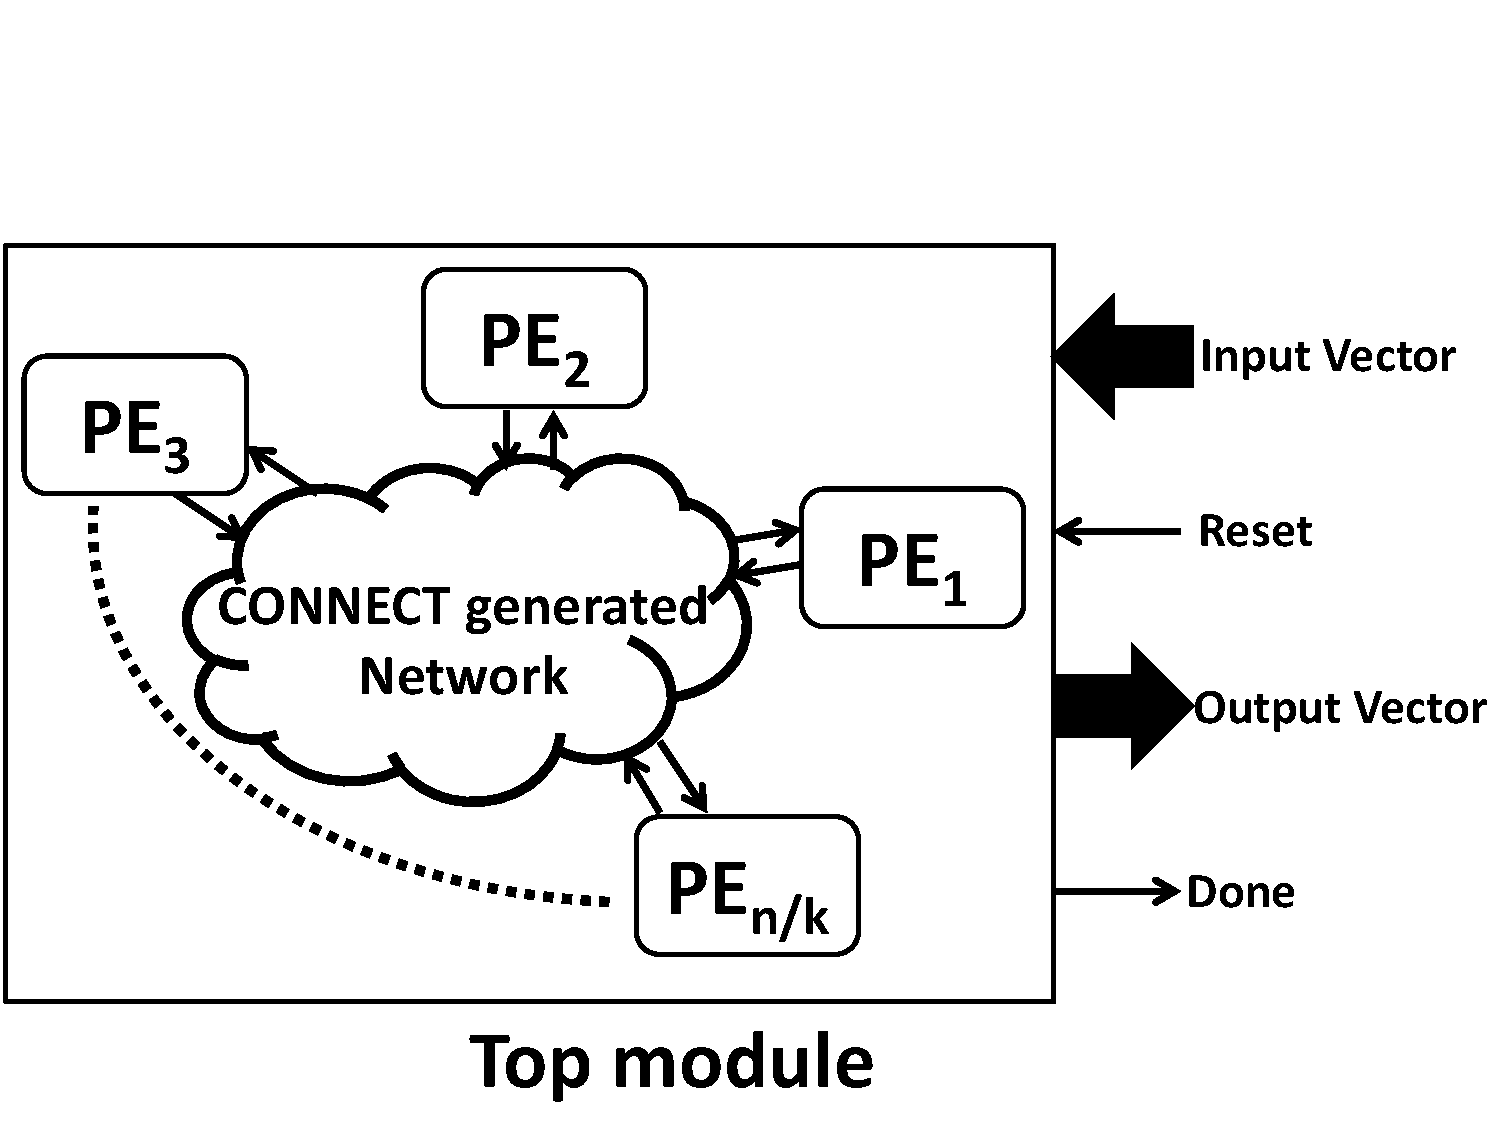
\includegraphics[scale=1, width=10cm]{figs/mult_top.pdf}
\caption{Top module for Boolean Matrix Vector Multiplication (BMVM).}
\label{fig:mult_top}
\end{figure}

In our approach, we observe that the behaviour of the network after in each iteration would be exactly identical if the PEs are exactly synchronized. Therefore, if we know the maximum number of cycles required for a PE to complete an iteration, all PEs could wait to synchronize at this cycle count after every iteration, thereby eliminating the need for additional broadcast messages. It is important to note that this count is dependent on the topology and routing policy used. We specify the count as a parameter to the processing element in our design, which could be determined by the user by simulating one iteration of the multiplication on the software. Our processing elements display the cycle counts at which the processing elements are done with one iteration (when they have sent and received all messages pertaining to that iteration), and the maximum of this count can be specified in that parameter. The source code of our processing element is included in~\ref{•}. Other parameters used by this module are 
specified and explained in~\ref{•}. Figure~\ref{fig:mult_top} shows the top level user module along with their module names in our design, consisting of several instances of processing elements connected by a CONNECT generated NoC. It must be noted that the NoC can itself be partitioned using our script, in which case the top module would consist of multiple instances for NoC corresponding to different partitions, with serial wire and flow control signals between them. We have only tested our partitioned NoC for boolean vector multiplication on a single FPGA, with wires corresponding to different partitions connected internally. Since the partitioned NoC itself has been tested successfully on separate Virtex 5 boards, we believe that multiplier design should also work for multi-FPGA case. The interface to the top module is kept as simple as providing the input vector followed by a reset signal as input, and obtaining the output vector on the done signal at the output.\\

In our final step, we wish to encapsulate our multiplication hardware within a software library to make it usable for target applications, mostly running on software. For this purpose, we use Reusable Integration Framework for FPGA Accelerators (RIFFA 2.0)~\cite{jacobsen2013riffa}, which provides a simple open-source integration framework for FPGA-CPU communication over high-speed PCIe links. On the software end, RIFFA provides a simple API to open/close an FPGA connection, send/receive data from FPGA and to send reset the FPGA user module. Although we use a single channel (corresponding to network sockets and parallel user cores), RIFFA can support upto 12 channels. The data transfers in RIFFA occur through PCIe transactions, with FPGA acting as the DMA bus master. For more details, the reader can refer to~\cite{jacobsen2013riffa}. \\

\begin{figure}[t!]
\centering
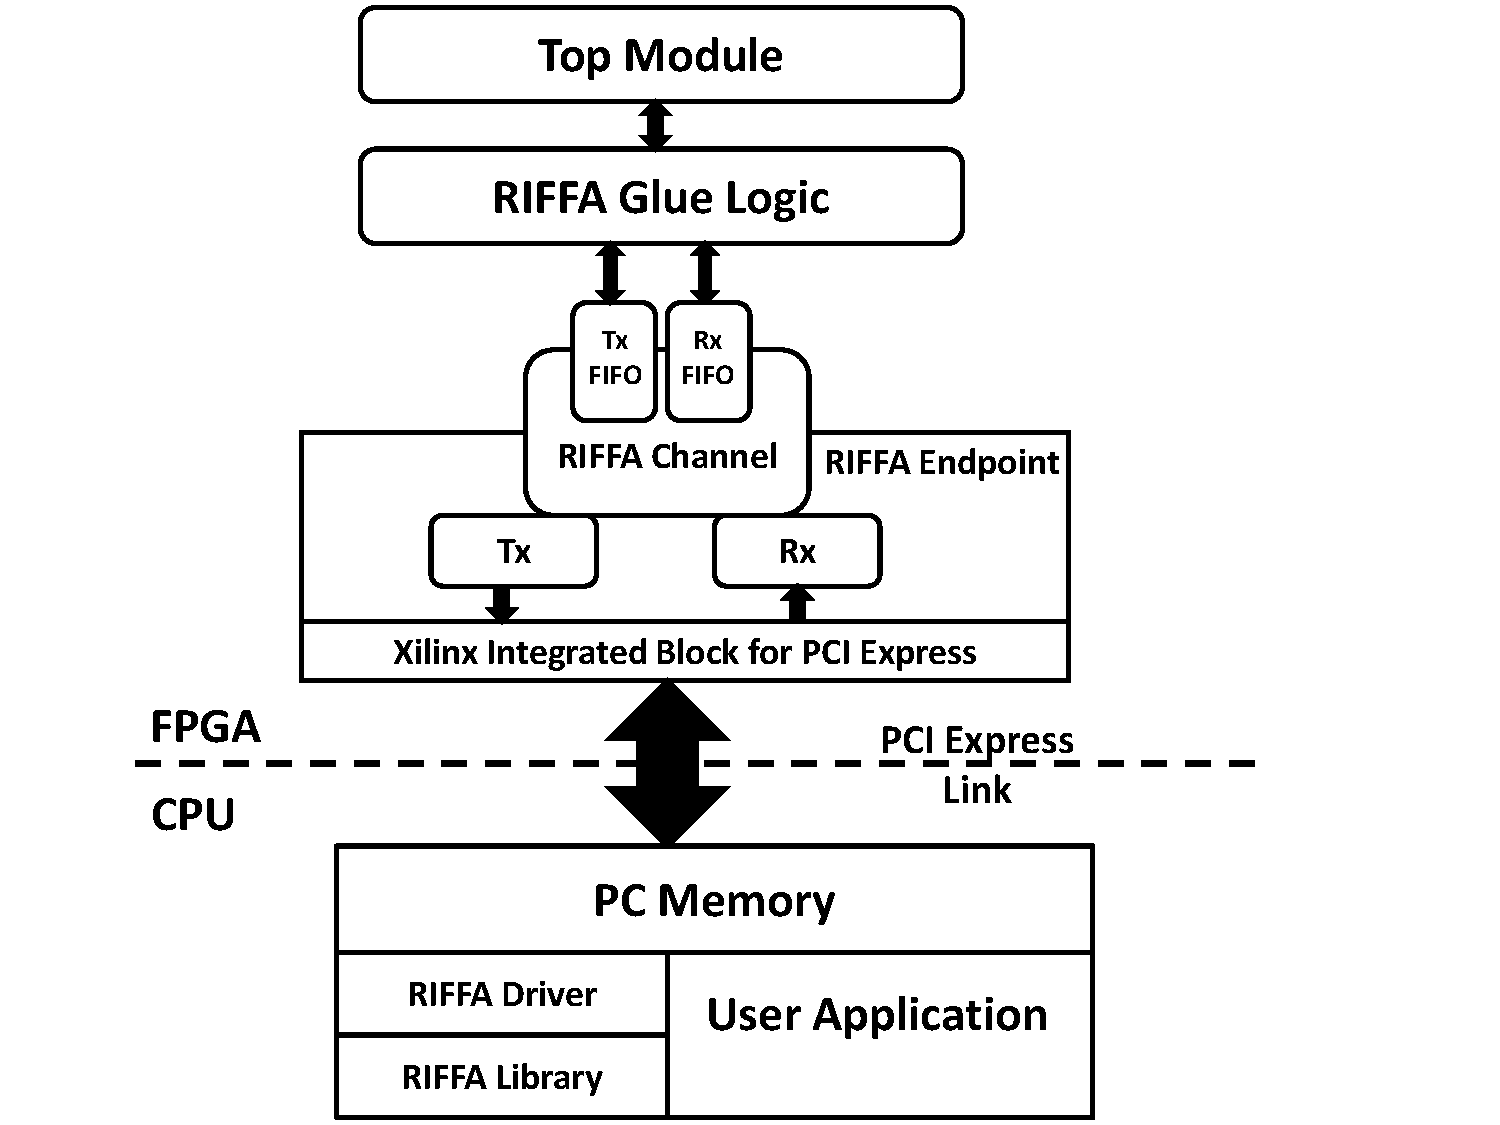
\includegraphics[scale=0.35]{figs/riffa.pdf}
\caption{BMVM framework with RIFFA.}
\label{fig:riffa}
\end{figure}

We demonstrate the usage using a simple C application shown in ~\ref{•}. The application resets the FPGA and sends an input vector, on which the multiplication is performed by the FPGA, before waiting to receive the output product. Since the application is written for a 32-bit processor, appropriate precautions are taken to make it compatible with the \emph{little endianess} of the RIFFA hardware modules supporting 64-bits. We also implement the necessary glue logic for the hardware interface between RIFFA endpoint and multiplier module as shown in Figure~\ref{fig:riffa}. The code for this module is available in ~\ref{•}.\\  
      
\subsection{Software implementation}

For comparison, we have also implemented a multi-threaded software implementation of the described boolean matrix vector multiplication (BMVM). The source code is available in ~\ref{•}. A shared memory model, using the \emph{pthread} library is used , in which a thread is an exact equivalent of the processing element in the FPGA. The input parameters to the application include the input matrix size, number of parallel threads, size of look-up per vector (sub-vector size to the power of $2$), folding factor and the number of iterations. The threads are first initialized with look-up tables, generated using the MATLAB code as described earlier in the section, and are also provided with the input sub-vector. Since multiple parallel threads may try to update the same sub-vector at once leading to concurrency issues described earlier, mutual exclusion between parallel updates is ensured using \emph{locks}. All the threads are also required to synchronize on a \emph{barrier}, before proceeding to the next 
iteration. Our implementation, in its current form, is naive and has scope for improvement. For instance, an entire 32-bit integer is allocated for a single bit in a matrix/vector, although bit-level operations are also possible in most processors. However, even with these software level optimizations, we do not expect the application speedup by more than a few factors.


\section{Conclusion and Future work}
\bibliographystyle{IEEEtran}
% argument is your BibTeX string definitions and bibliography database(s)
\bibliography{IEEEabrv,ref}

% that's all folks
\end{document}


